\documentclass[a4paper]{article}
\title{House preference model}
\author{Beichen Su, ID:904882814}
\usepackage{amsmath}
\usepackage{Sweave}
\usepackage[framed,numbered,autolinebreaks,useliterate]{mcode}
\usepackage{graphicx}
\graphicspath{ {images/} }
\begin{document}
\Sconcordance{concordance:project_tex.tex:project_tex.Rnw:%
1 34 1 1 2 1 0 2 1 19 0 2 2 1 0 1 1 11 0 1 2 1 0 1 2 4 0 1 2 1 4 3 0 1 %
1 1 9 11 0 2 2 1 0 5 1 3 0 1 2 2 1 1 2 5 0 1 3 5 0 1 2 3 1 1 2 1 0 2 1 %
1 3 5 0 1 4 6 0 1 3 1 0 2 1 1 2 1 0 1 1 4 0 1 2 3 1 1 2 10 0 2 1 23 0 1 %
2 20 1 1 2 1 0 1 1 1 2 1 0 2 1 11 0 4 1 4 0 1 2 87 1}

\maketitle

\section{Introduction}
As I am looking for my apartment to rent for the next year, I observed that it cost some time so find a place that exactly meet my desire. So that I intended to build a optimization model for each person to find their own house based on their own consideration of characteristics of an apartment, such as the price, the safety level, and the location from their office or school. Observing that apartments in same area share something in common, I am going to analysis this trend for characteristics of houses. For this report, the focus is on the price of rentals.


\section{Assumptions}
To approach this model, I made some assumptions.\\
To begin with, I assume that rentals can be found anywhere on the map for there is a pair of longitude and latitude everywhere on the map during regression. So that I have to include them for regression but they are actually meaningless.\\
Secondly I assume the earth is not a sphere and treat the longitude and latitude as x,y coordinate on a flat plane, which makes it possible to draw grids and this approximation won't lose too much accuracy in a small area.\\


\section{Model}
Below I introduce my optimization model:\\
$Minimize: w_1 * \frac{|Price_{Desired} - Price_{Real}|}{Price_{Desired}} + w_2 * \frac{|Crime rate_{Desired} - Crime rate_{Real}|}{Crime rate_{Desired}}.........$\\

where $\sum w_i = 1$ is representing the weight for each factor, all factors are put on same scale and this optimization subjects to longitude and latitude.\\
This will return an ideal longitude and latitude for a individual to look for his or her desired apartment. 

\section{Sub-model(Price)}
Here it takes several steps to get a clean data that I'd like to investigate.

\subsection{Row data and zipcode searching method}
For easy data access, I choose the price as the factor for investigate. There are some data sets on Zillow to investigate and I choose this ZRI(Zillow rental index table) which represent the median rent price in the specific area, including all house type for a given zip-code.\\
Here I obtained the ZRI for the current month.
\begin{Schunk}
\begin{Sinput}
> setwd("C:/Users/subei_000/Desktop/404 Project")
> mydata = read.csv("zillow.csv")
> head(mydata)
\end{Sinput}
\begin{Soutput}
       Date RegionName State    Metro   County     City SizeRank  Zri
1 2017/1/31      10025    NY New York New York New York        0 3556
2 2017/1/31      60657    IL  Chicago     Cook  Chicago        1 1890
3 2017/1/31      10023    NY New York New York New York        2 3840
4 2017/1/31      60614    IL  Chicago     Cook  Chicago        3 2129
5 2017/1/31      79936    TX  El Paso  El Paso  El Paso        4  992
6 2017/1/31      10002    NY New York New York New York        5 3656
           MoM          QoQ         YoY ZriRecordCnt
1 -0.003083824 -0.009194762 -0.01767956        22431
2 -0.010471204 -0.030769231 -0.03669725        32224
3 -0.002597403 -0.019157088 -0.01865576        29114
4 -0.006532898 -0.023394495 -0.05461812        33150
5 -0.001007049 -0.007007007 -0.04889741        31486
6 -0.009214092 -0.028434760 -0.02636485         9172
\end{Soutput}
\end{Schunk}
It's possible to locate the price by longitude and latitude on map, by searching the zip-code from an zip-code and location table.
\begin{Schunk}
\begin{Sinput}
> ZLL = read.csv("zipcode.csv")
> head(ZLL[,1:7])
\end{Sinput}
\begin{Soutput}
  Zipcode ZipCodeType     City State LocationType   Lat   Long
1     705    STANDARD AIBONITO    PR      PRIMARY 18.14 -66.26
2     610    STANDARD   ANASCO    PR      PRIMARY 18.28 -67.14
3     611      PO BOX  ANGELES    PR      PRIMARY 18.28 -66.79
4     612    STANDARD  ARECIBO    PR      PRIMARY 18.45 -66.73
5     601    STANDARD ADJUNTAS    PR      PRIMARY 18.16 -66.72
6     631      PO BOX CASTANER    PR      PRIMARY 18.19 -66.82
\end{Soutput}
\begin{Sinput}
> # Load zipcode of the real data points
> zipcode = mydata$RegionName
> # Load the ZRI of the real data points
> ZRI = mydata$Zri
\end{Sinput}
\end{Schunk}
Here's the search step.
\begin{Schunk}
\begin{Sinput}
> # Find the longitude and latitude of those points
> # If cannot find the longitude and latitude, set -1 indicating no found
> longitude = c()
> latitude = c()
> for (i in 1:15916) {
+   if (length(ZLL[which(ZLL$Zipcode == zipcode[i]),]$Long) > 0) {
+     longitude[i] = ZLL[which(ZLL$Zipcode == zipcode[i]),]$Long
+     latitude[i] = ZLL[which(ZLL$Zipcode == zipcode[i]),]$Lat
+   } else {
+     longitude[i] = -1
+     latitude[i] = -1
+   }
+ }
\end{Sinput}
\end{Schunk}
Below I removed those original points without an location associated with them.
\begin{Schunk}
\begin{Sinput}
> RTR = which(latitude == -1)
> ZRI = ZRI[-RTR]
> longitude = longitude[-RTR]
> latitude = latitude[-RTR]
> zipcode = zipcode[-RTR]
> newData = cbind(ZRI,zipcode,longitude,latitude)
\end{Sinput}
\end{Schunk}

\subsection{Some plots and data reduction}
By now I have 15913 ZRI associated with their longitude and latitude.
\begin{Schunk}
\begin{Sinput}
> plot(longitude,ZRI, main = "ZRI vs longitude")
\end{Sinput}
\end{Schunk}
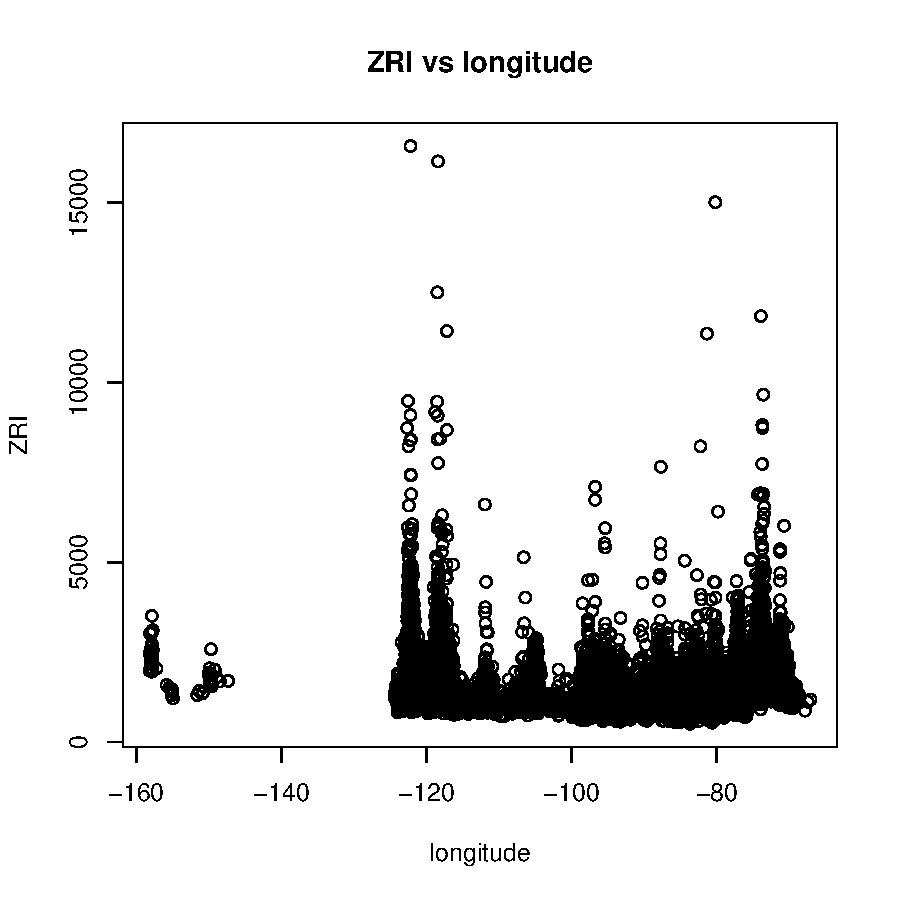
\includegraphics{project_tex-test1}
\begin{Schunk}
\begin{Sinput}
> plot(latitude, ZRI, main = "ZRI vs latitude")
\end{Sinput}
\end{Schunk}
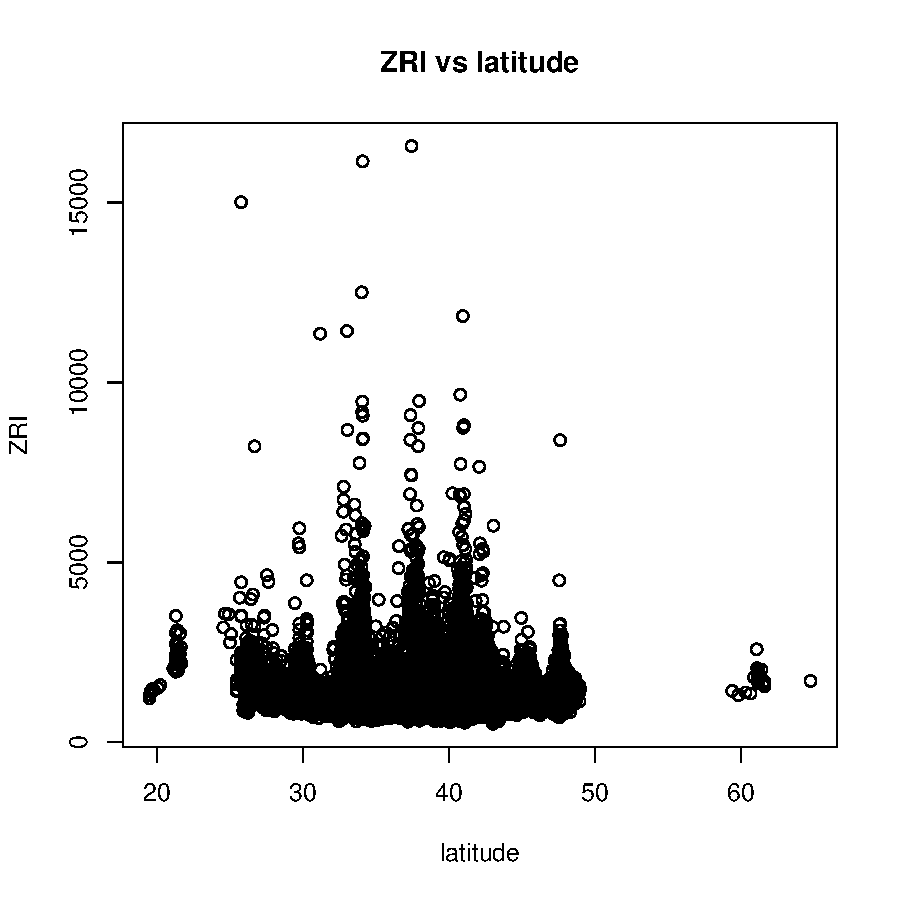
\includegraphics{project_tex-test2}


There are one clusters of data points appearing to be outliers in both plot. It's easy to identify them as the gap in longitude and latitude suggest them as Hawaii and Alaska. For these gaps affects the regression, I drop them off and focus on the continent of USA.\\
Below I present the plots for the new data. 
\begin{Schunk}
\begin{Sinput}
> RTRlati = which(latitude >50)
> RTRlong = which(longitude < -125)
> newData = newData[-c(RTRlati,RTRlong),]
> plot(newData[,3],newData[,1],main = "ZRI vs longitude", 
+      xlab = "longitude", ylab = "ZRI")
\end{Sinput}
\end{Schunk}
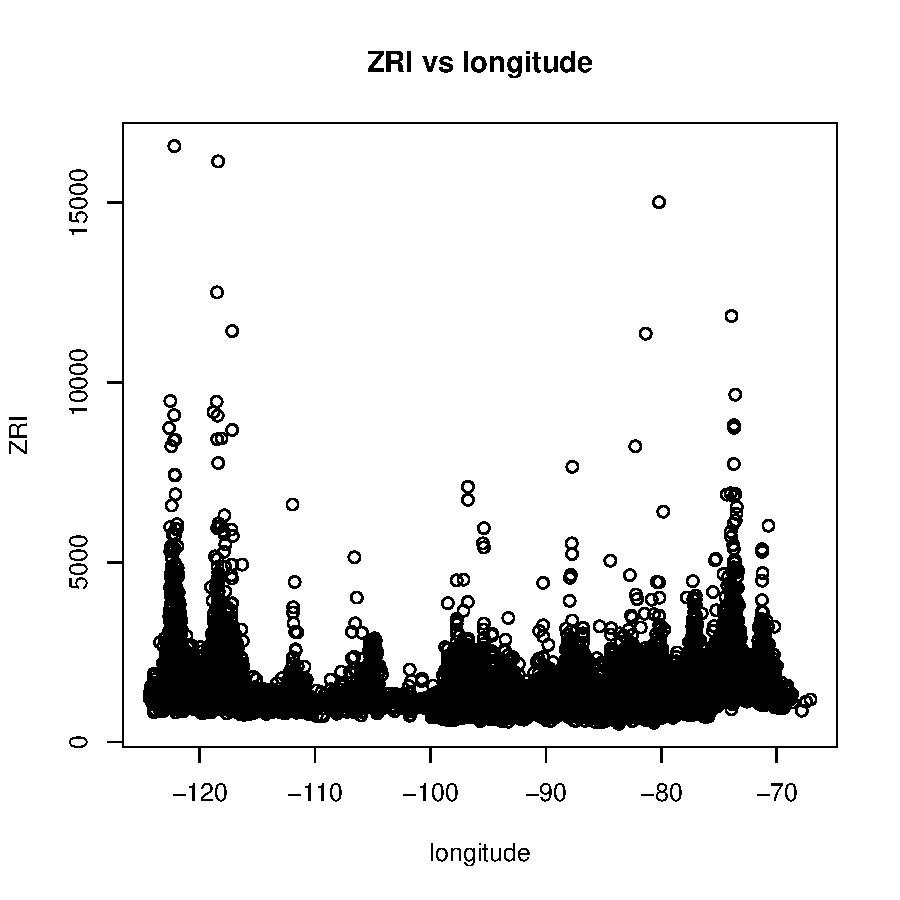
\includegraphics{project_tex-test3}
\begin{Schunk}
\begin{Sinput}
> plot(newData[,4],newData[,1],main = "ZRI vs latitude", 
+      xlab = "latitude", ylab = "ZRI")
\end{Sinput}
\end{Schunk}
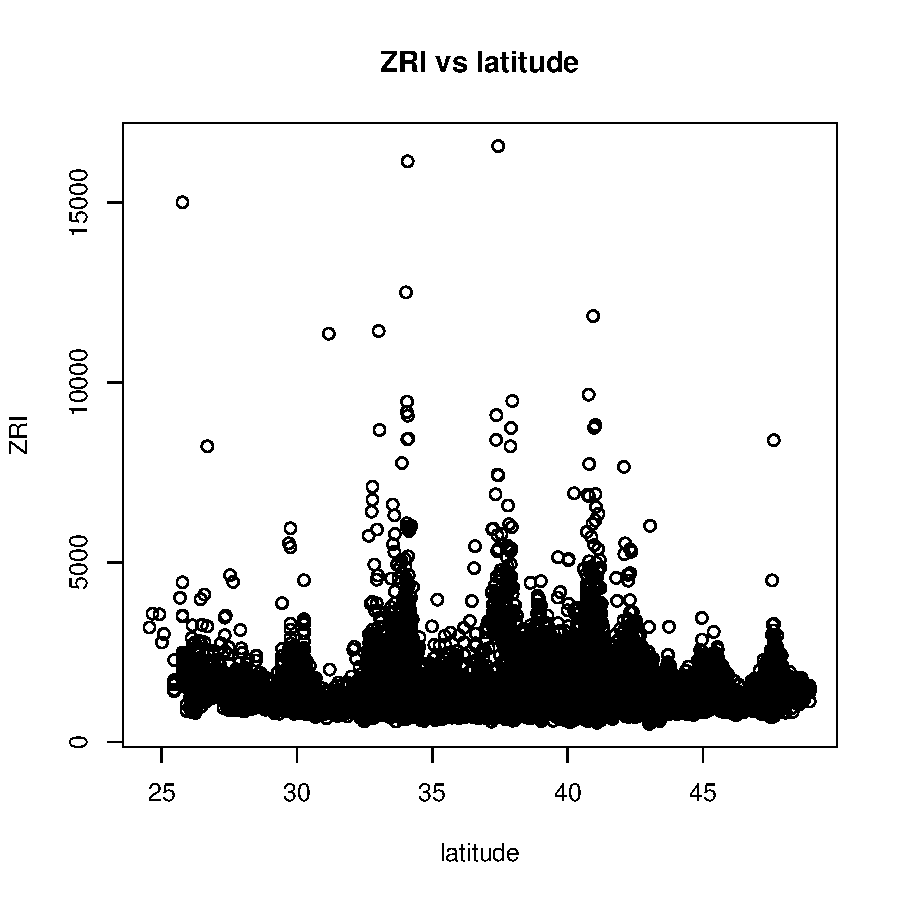
\includegraphics{project_tex-test4}
\begin{Schunk}
\begin{Sinput}
> library(rworldmap)
> library(sp)
> newmap <- getMap(resolution = "low")
> plot(newmap, xlim = c(-124,-66), ylim = c(25,48), 
+      asp = 2, main = ' All location recorded on map')
> points(newData[,3],newData[,4],col= 'red', cex = 0.2)
\end{Sinput}
\end{Schunk}
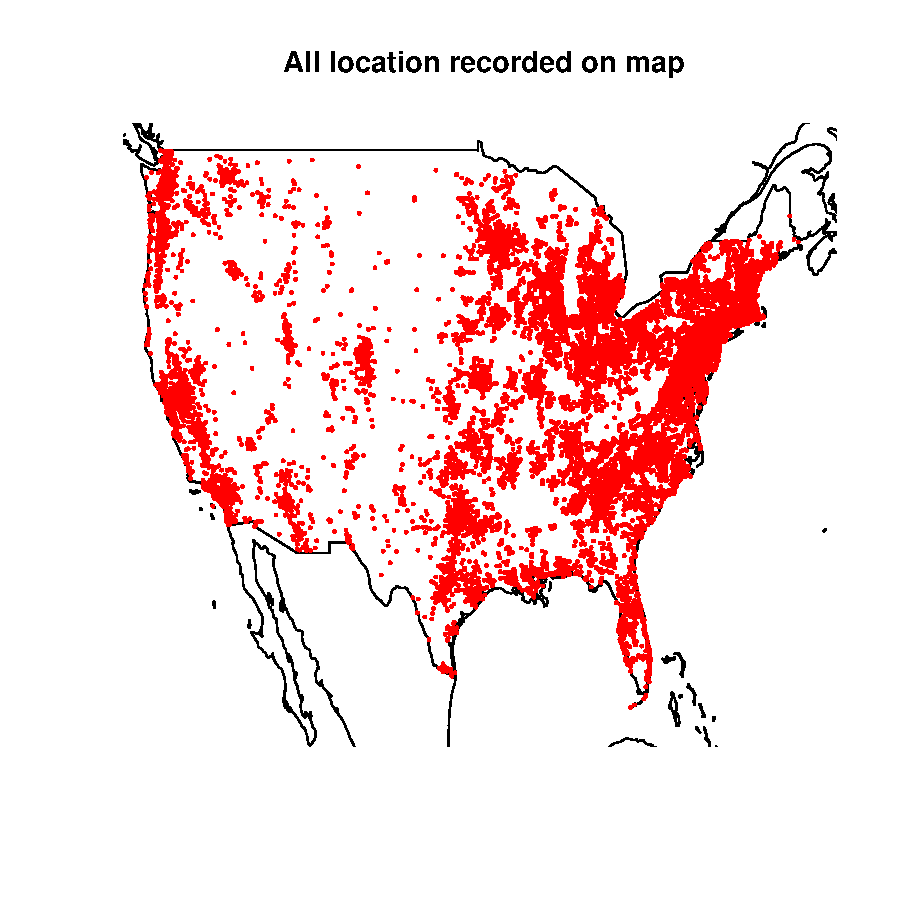
\includegraphics{project_tex-test5}


\subsection{Parametric method, linear regression}
Obtaining this set of clean data, I run a simple linear regression and check their correlation. $ZRI = \beta_{0} + \beta_{1}*longitude + \beta_{2}* latitude$\\
\begin{Schunk}
\begin{Sinput}
> cor(newData)
\end{Sinput}
\begin{Soutput}
                   ZRI     zipcode   longitude     latitude
ZRI        1.000000000  0.02690427 -0.12719215  0.002492236
zipcode    0.026904272  1.00000000 -0.94093425 -0.144937973
longitude -0.127192146 -0.94093425  1.00000000  0.063822432
latitude   0.002492236 -0.14493797  0.06382243  1.000000000
\end{Soutput}
\begin{Sinput}
> lfit = lm(newData[,1]~newData[,3]+newData[,4])
> summary(lfit)
\end{Sinput}
\begin{Soutput}
Call:
lm(formula = newData[, 1] ~ newData[, 3] + newData[, 4])

Residuals:
    Min      1Q  Median      3Q     Max 
 -960.1  -455.9  -203.8   215.2 14859.2 

Coefficients:
             Estimate Std. Error t value Pr(>|t|)    
(Intercept)  830.9847    63.0298   13.18   <2e-16 ***
newData[, 3]  -6.7283     0.4153  -16.20   <2e-16 ***
newData[, 4]   1.6977     1.2580    1.35    0.177    
---
Signif. codes:  0 '***' 0.001 '**' 0.01 '*' 0.05 '.' 0.1 ' ' 1

Residual standard error: 770.8 on 15852 degrees of freedom
Multiple R-squared:  0.01629,	Adjusted R-squared:  0.01617 
F-statistic: 131.3 on 2 and 15852 DF,  p-value: < 2.2e-16
\end{Soutput}
\end{Schunk}
The correlation matrix tells that the linear relationship between those 3 variables is weak, as well as the poor $R^2$ can tell.\\
It's not surprising that I get this result, because I am wondering the cluster of apartments with high ZRI are centered in each city and in 3D the ZRI should be a bump in each area, which suggests this parametric method might not work well for this sub-model.

\subsection{Non-parametric method, Kernel regression}
The idea of Kernel regression that takes ZRI as response variable and longitude and latitude as predictor variable can be approached by drawing grid points on the map and obtaining the kernel density estimation for each grid points given the original points. The formula is given below:\\
Define 
$V_{i,j}= \begin{pmatrix} 
m_{Xi}\\
m_{Yj}  
\end{pmatrix}$, and $O_{k}= \begin{pmatrix} 
X_{k}\\
Y_{k}  
\end{pmatrix}$, where $V_{i,j}$ stands for the $i^{th}$ row and $j^{th}$ column grid point to be estimated and $O_{k}$ stands for the $k^{th}$ original data points. The estimation is given by:\\
$\hat{f(V_{i,j})} = \frac{\sum_{k}^{n}K(\frac{\|V - O_{k}\|_{2}}{b})*Z_{k}}{\sum_{k}^{n}K(\frac{\|V - O_{k}\|_{2}}{b})}$\\
where K represents the Gaussian kernel and b the bandwidth.


\subsubsection{Data reduciton again}
The asymptotic analysis gives the kernel regression $O(N^3)$, which is actually very bad algorithm and impossible to run with 15855 data points insides the first of 3 loops. So that I can only apply this algorithm in a small area.
As 0.001 change in longitude approximately represent a distance of one block on map, I can't define my grid too wide, which is meaning less, for this calculation I set the grid on longitude and latitude seperated by 0.01.
I pull out the original points in a rectangle area, from -80.94 to -73.50 for longitude and 37.57 to 40.75 for latitude, including Washington.D.C in the middle and New York in the right top corner. Below I present the data points on the map.
\begin{Schunk}
\begin{Sinput}
> RTKlong = which(newData[,3] < -73.50 & newData[,3] > -80.94)
> TTemp = newData[RTKlong,]
> # Filter out the row by new defined latitude
> RTKlati = which(TTemp[,4] > 37.57 & TTemp[,4] < 40.75)
> SData = TTemp[RTKlati,]
> head(SData)
\end{Sinput}
\begin{Soutput}
      ZRI zipcode longitude latitude
[1,] 3556   10025    -73.99    40.71
[2,] 3840   10023    -73.99    40.71
[3,] 3656   10002    -73.99    40.71
[4,] 2179   11226    -73.94    40.64
[5,] 2145   11375    -73.84    40.72
[6,] 3652   10016    -73.99    40.71
\end{Soutput}
\begin{Sinput}
> b = bw.nrd(sqrt(SData[,3]^2 + SData[,4]^2))
> newmap <- getMap(resolution = "low")
> plot(newmap, xlim = c(-80.94,-73.50), ylim = c(37.57,40.75), asp = 2, main = 'Location recorded on map around Washington D.C')
> points(SData[,3],SData[,4],col= 'red', cex = 0.6)
\end{Sinput}
\end{Schunk}
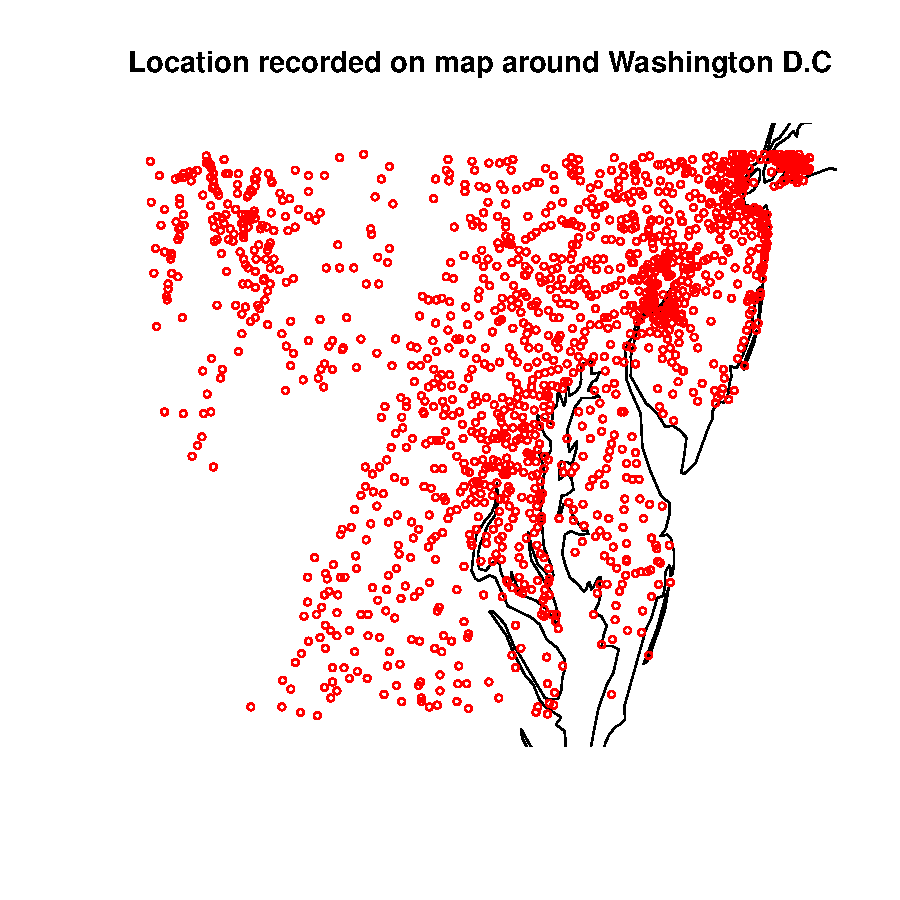
\includegraphics{project_tex-test6}

\subsubsection{Kernel regression and result}
Now I pull this data out to Matlab for kernel regression and visualization. Here's the matlab code and contour plot:\\

\begin{lstlisting}
clear all;close all; clc
load smallData.txt;
z = smallData(:,1);
x = smallData(:,3);
y = smallData(:,4);
%scatter(x,y)
gx = (min(x):0.01:max(x));
gy = (min(y):0.01:max(y));
b = 0.331627;
p = length(gx);
q = length(gy);
n = length(x);
result = zeros(742,317);
for i = 1:p
    for j = 1:q
        a1 = 0;
        a2 = 0;
        for k = 1:n
            u = sqrt((x(k) - gx(i))^2 + (y(k)-gy(j))^2)/b;
            c = 1/(sqrt(2*pi))*exp(-0.5*(u^2))/b;
            a1 = a1 + z(k)*c;
            a2 = a2 + c;
        end
        result(i,j) = a1/a2;
    end
end
[X,Y] = meshgrid(gx,gy);
result = transpose(result);
h = surface(X,Y,result);
set(h,'LineStyle','none')
xlswrite('FinalData.xlsx',result);
[C,h] = contour(X,Y,result);   
clabel(C,h)

final = zeros(p*q,3);
count = 0;
for i  = 1: 317
    for j = 1:743
        count = count + 1;
        final(count,1) = result(i,j);
        final(count,2) = X(i,j);
        final(count,3) = Y(i,j);
    end
end
xlswrite('FFinalData.xlsx',final);
\end{lstlisting}

Also, I rearrange the format of the outcome matrix. It's originally a matrix with value on each grid points and I extract the estimated ZRI with it's corresponding longitude and latitude and form a k X 3 matrix, where K is the $K^th$ point of estimation. After this I output the rearrange matrix to an xlsx file and use it in R to generate a heat plot.

\subsubsection{Visualization}
First I attached this part of map by ggmap. To run this tex file faster I just attach the picture rather than run the ggmap code in this tex file.\\
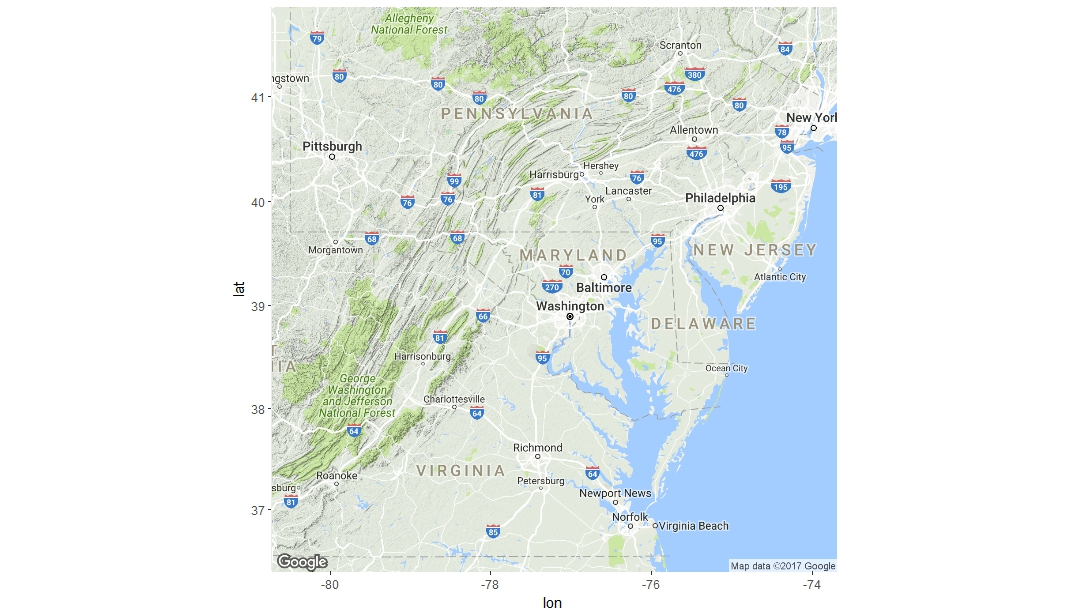
\includegraphics[width=15cm,height=15cm,keepaspectratio]{Rplot}\\
Now I have a contour plot from Matlab:\\
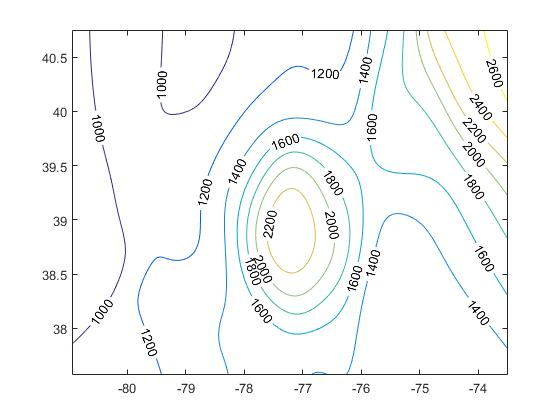
\includegraphics[width=15cm,height=15cm,keepaspectratio]{contour}\\
Which clearly shows that there are two peaks of ZRI on Washington D.C and New York.\\
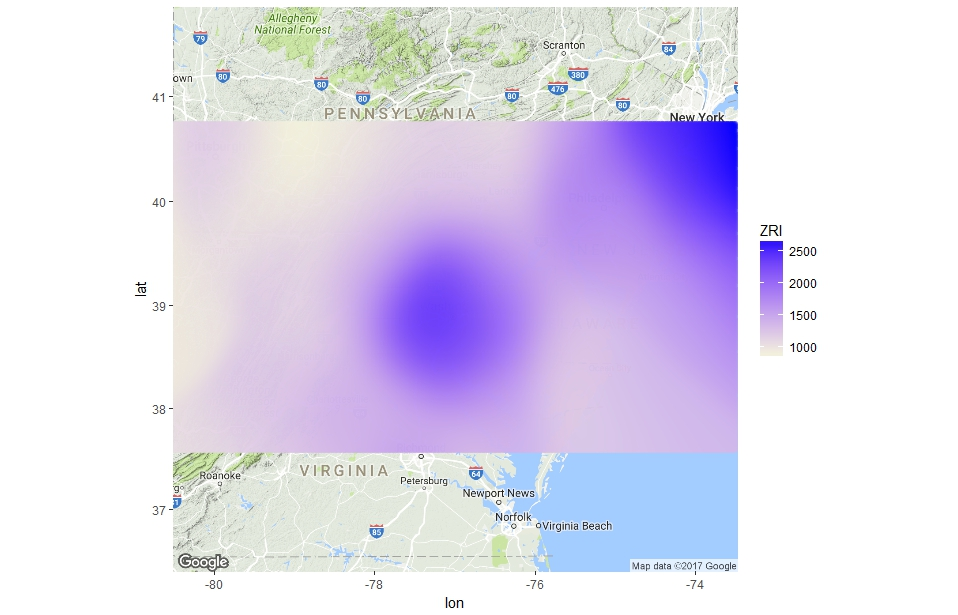
\includegraphics[width=15cm,height=15cm,keepaspectratio]{heatmap}\\
And finally a heat map generated by ggmap in R. It shows the same result.

\subsubsection{Interpretation and discussion}
The graphs above show that the kernel regression works pretty well as it identifies the place with high ZRI and it can actually return a estimation for ZRI given a certain longitude and latitude.\\
But a confidence interval is better than a single estimation. However the bootstrap confidence interval can be approached ideally but based on an $O(N^3)$ algorithm I dont't think my laptop can complete this task.\\
Afterall, the kernel regression is powerful for some obvious non-linear pattern, such as the price of rental shows as peaks on map. And it's extremely useful for a small area, for reduced work load and smaller grid that would improve its accuracy.\\
As for the data chosen, the ZRI only represnt the median rental price of a certain area, and I think it's better to distinguish the house type, such as studio, 1-bedroom and more. This would improve the users' experience for the big optimization model but the data sets for these seperated type is limited and I don't think they are enough to build a kernel regression.\\
As the big optimation suggests, there are more factors to add in and minimize the difference for the preferred and exact characteristics. If supported with enough data, the big optimization model can be acheived by kernel regression for a specfic area and would provide some helpful suggestion for customers who are looking for rentals.


















\end{document}
